\documentclass[main.tex]{subfiles}
\begin{document}
\newpage
\section{Telegrafenrauschen in Samarium-Erbium-Orthoferrit}

\todo{Roter Faden!}
\todo{Überschriften}
\todo{gibt es offizielle namen für die verwendeten Eigenbezeichnungen?}
\todo{mehr direkte refernezen auf Plots}

\todo{Einleitung und Beschreibung \cref{fig:bsp-run}}

Der betrachtete Orthoferrit besteht aus vier Untergittern, welche jeweils eine andere Gleichgewichtsmagnetisierung \(\vec{S}_i\) besitzen. Im nachfolgenden Bereich wird die normierte resultierende Magnetisierung (Überlagerung der vier Untergitter) verwendet.

\begin{align}
    % \mu_{1} &=  \mu_{2} = \mu_{3} = \mu_{4} = \num{3.66}\mu_B \\
    \vec{m} &= \frac{1}{4} \sum_{i=1}^4 \vec{S}_i
\end{align}

Das Telegrafenrauschen tritt am untersuchten Reorientierungsübergang (siehe \cref{fig:bc-crit-temp}) in c-Richtung auf, weshalb nur diese Komponente betrachtet wird.

% Eine Simulation, von einem \(192 \times 192 \times 192\) Gitter mit einem simulierten Zeitraum von \qnt{1.2}{\nano\second} mit einer numerischen Schrittweite von \qnt{20}{\femto\second} benötigt etwa drei Tage Rechenzeit auf einer Nvidia RTX 2080 Ti Grafikkarte. 

In diesem Simulationszeitraum sind im optimalen Temperaturbereich (um mehrere eindeutige Schaltvorgänge zu beobachten) etwa 15-25 Schaltvorgänge pro Simulation zu beobachten vgl. \cref{fig:bsp-run}

Um mehr Schaltvorgänge pro Simulation betrachten zu können, wurde der Simulationszeitraum teilweise verdoppelt.

\begin{figure}[h]
    \centering
    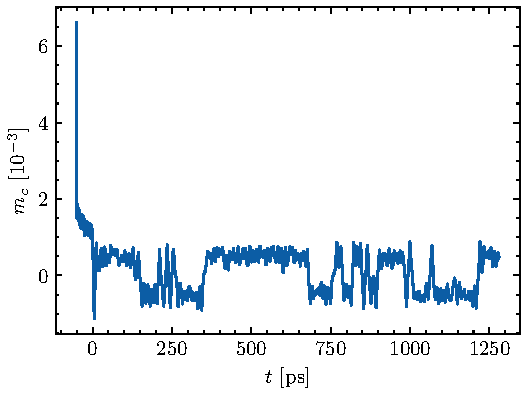
\includegraphics{bilder/plots/theo-vis/example-telegraph-sim.pdf}
    \caption{Einzelne Simulationskurve von \(m_c\) bei \(T \approx \qnt{302}{\kelvin}\). Im Zeitraum \(<0\) ist hierbei die Equilibrierung zu sehen
    }\label{fig:bsp-run}
\end{figure}

\subsection{Extraktion des Telegrafenrauschens}

Um das Telegrafenrauschen zu extrahieren wird der Algorithmus \cref{sec:algo} angewandt.
Das Histogramm über das die Zustände bestimmt werden, ist in \cref{fig:extraktion-tgr} rechts zu sehen. Auf dem kurzen intervall ist bereits gut erkennbar, dass die doppelte Gausverteilung den Bereich zwischen den zwei Niveaus nicht gut beschreibt. In \cref{fig:fit_func_comp} wird versucht mithilfe einer Anderen Verteilungsfunktion die Wahrscheinlichkeitsdichteverteilung zu fitten.

\begin{figure}[H]
    \centering
    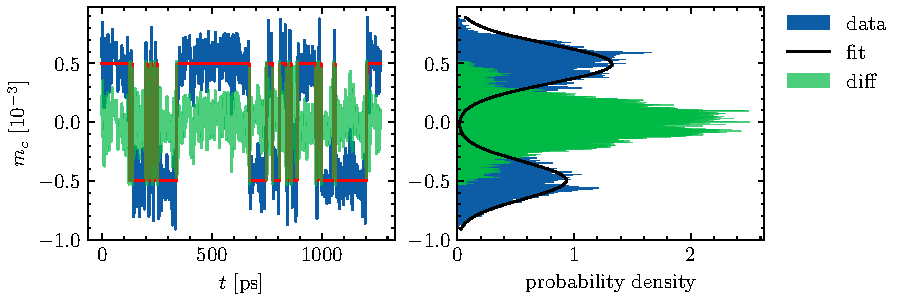
\includegraphics{bilder/plots/Bz_0mT/mc_fit_hist_part2_26.03meV.pdf}
    \caption{Extraktion des Telegrafenrauschen mithilfe des Algorithmus aus \cref{sec:algo}. Die Fitfunktion im rechten Plot ist dabei ein doppelter Gauss-Peak über den den die Intervalle der beiden Zustände bestimmt werden. Das bereinigte Telegrafenrauschen ist im linken Plot in rot zu sehen.\todo{in Legende hinzufügen} Die Differenz zwischen bereinigtem Telegrafenrauschen und dem rohen Signal ist in grün zu sehen.}\label{fig:extraktion-tgr}
\end{figure}

Die Aufenthaltswahrscheinlichkeit zwischen den zwei Zuständen ist deutlich größer, als bei zwei überlagerte Gaußverteilungen anzunehmen wäre. Bei Zwei Lorenzverteilungen ist die Aufenthaltswahrscheinlichkeit im Randbereich jedoch gar nicht passend.

\begin{figure}[H]
    \centering
    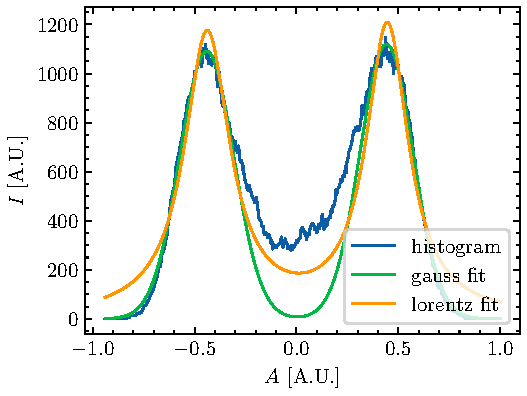
\includegraphics{bilder/plots/theo-vis/hist_fit_comp.pdf}
    \caption{Vergleich von verschiedenen Verteilungsfunktionen um die Wahrscheinlichkeitsdichte $P(m_c)$ zu fitten.}\label{fig:fit_func_comp}
\end{figure}

Theoretisch müsste auch noch ein dritter, instabiler, Zustand existieren (Lokales maximum), der genau zwischen den zwei Niveaus liegt. Dieser sorgt für die Abweichung von einer Gaußverteilung im Bereich zwischen den zwei Niveaus. \todo{Etwas weniger schwammig formulieren}

Um diesen Zustand auch charakterisieren zu können wäre ein deutlich komplexerer Algorithmus notwendig. Außerdem ist die Aufenthaltswahrscheinlichkeit doch verhältnismäßig klein, weshalb er hier nicht weiter betrachtet wird.

\subsection{Einfluss verschiedener Temperaturen}

% Das Telegrafenrauschen tritt ja nur an der Reorientierungstemperatur auf. 
% Daher wird die Temperatur varriert, um zu beobachten, wie das Telegrafenrauschen entsteht und wieder verschwindet.

Im Rahmen der Masterarbeit von Julius Schlegel \cite{schlegel-master} wurden bereits Simulationen für verschiedene Temperaturen durchgeführt. Diese Daten wurden für diesen Teil der Analyse verwendet

\subsubsection{Betrachtung in der Zeitdomäne}

Da aus der Simualation das Rauschsignal direkt gewonnen werden kann, bietet es sich an dieses statistisch zu untersuchen.

\begin{figure}[H]
    \centering
    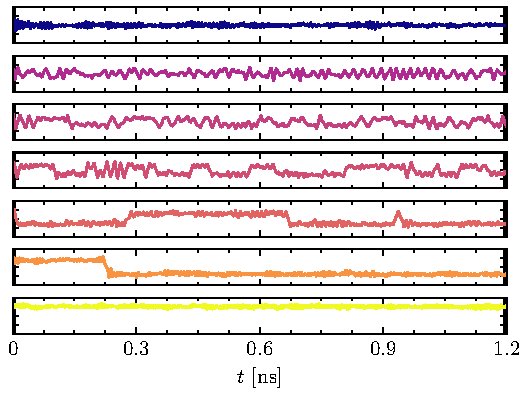
\includegraphics{bilder/plots/temp_comparison_long/mc_time.pdf}
    \caption{\(m_c\) im Zeitlichen Verlauf für verschiedene Temperaturen. Die Daten sind jeweils aus einem einzelnen Simulationslauf. Die Colormap ist hierbei identisch zu der in \cref{fig:temp-hist}. Die y-achse reicht jeweils von \num{-2e-3} bis \num{+2e-3}}\label{fig:temp-time}
\end{figure}

Unterhalb von \qnt{300}{\kelvin} existiert nur ein einzelner Zustand, um den \(m_c\) fluktuiert. Je höher die Temperatur wird, desto stärker bilden sich die beiden Zustände aus und das Telegrafenrauschen wird deutlicher sichtbar. Wenn die Temperatur weiter erhöht wird, ist die mittlere Aufenthaltszeit irgendwann\todo{Genauer} größer als der Simulationszeitraum und kann kein Schaltvorgang mehr beobachtet werden.


\begin{figure}[H]
    \centering
    \subcaptionbox{Temperaturbereich mit sichtbarem Telegrafenrauschen \label{fig:temp-hist-tg}}{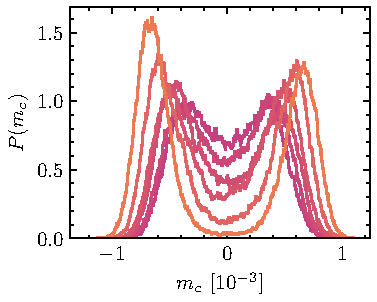
\includegraphics{bilder/plots/temp_comparison_long/mc_hist_tgr.pdf}}
    \subcaptionbox{größerer Temperaturbereich um den Reorientierungsübergang \label{fig:temp-hist-long}}{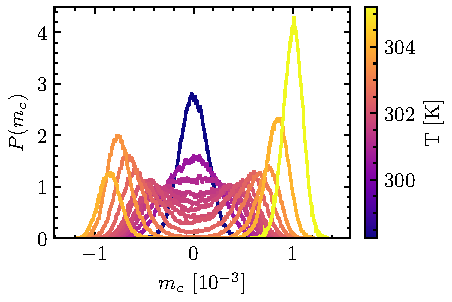
\includegraphics{bilder/plots/temp_comparison_long/mc_hist.pdf}}
    \caption{Wahrscheinlichkeitsdichteverteilung von \(m_c\) für eine Kombination von mehreren Simulationsläufen.}\label{fig:temp-hist}    
\end{figure}

Da die mittlere Aufenthaltszeit  für hohe Temperaturen ähnlich groß, wie der Simulationszeitraum ist, ist die Wahrscheinlichkeitsdichte der beiden Zustände (in den Simulationsdaten) hier teilweise stark unterschiedlich.
Aus theoretischer Sicht sollten die beiden Niveaus für die gelb-orangenen plots in \cref{fig:temp-hist} gleich groß sein. Aufgrund der kurzen Simulationszeit und der geringen Anzahl an Schaltvorgängen, ist dies hier aber nicht der Fall.

Da der Einschwingvorgang mit einem positiven Startwert (was \(m_c\) angeht beginnt, landet das System immer zuerst im oberen Niveau. Bei den Temperaturen oberhalb von \qnt{305}{\kelvin}, wechselt es nichtmehr von dort nicht ins untere Niveau. 

\begin{figure}[H]
    \centering
    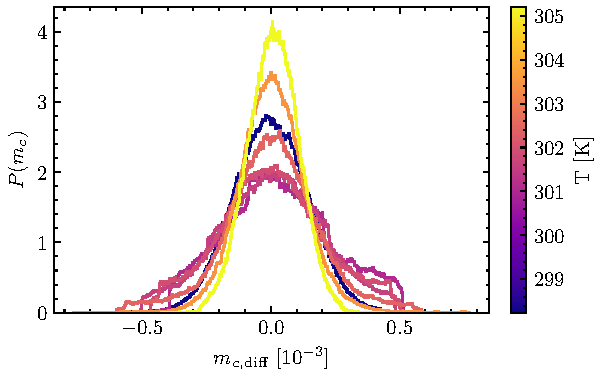
\includegraphics{bilder/plots/temp_comparison_long/mc_diff_hist.pdf}
    \caption{Wahrscheinlichkeitsdichteverteilung für Differenz zwischen rohem Signal und extrahiertem Telegrafenrauschen von \(m_c\) (entspricht extrahiertem statistisches Rauschen)}\label{fig:temp-diff-hist}    
\end{figure}

Bei einer Erhöhung der Temperatur wird also der Abstand der Zwei Zustände größer und ein Wechsel seltener. Doch welchen Einfluss hat dies auf die Verteilung des restlichen statistischen Rauchens?

Wenn vom rohen Signal das Telegrafenrauschen abgezogen wird (oder der Mittelwert, wenn nur ein Zustand existiert), bleibt ein statistisches Rauschen übrig, dessen Histogramm einer Gaußverteilung entspricht \cref{fig:temp-diff-hist}. \todo{Das sieht man nicht so einfach. fit hinzufügen?}

\todo{<genauer erklären>}Anhand der Abweichung von einer Gausverteilung im Randbereich (Sprünge statt kontinuierlicher Übergang) sind die Schwellenwerte, die der Algorithmus für die Zustände bestimmt hat, erkennbar.

Diese Verteilung ist für den Temperaturbereich mit aktivem Telegrafenrauschen deutlich breiter, als oberhalb und unterhalb. Dies Liegt wahrscheinlich auch vorallem an den Datenpunkten im Bereich zwischen den zwei Zuständen, welche nicht von der Gausverteilung beschrieben werden (siehe \cref{fig:fit_func_comp}).\todo{</genauer erklären>}
Interessanterweise verändert sich diese Verteilung in diesem Temperaturbereich nicht signifikant.\todo{viel genauer erklären}

Nachfolgend werden meist nur noch die 6 simulierten Temperaturen mit klar erkennbarem Telegrafenrauschen betrachtet (vgl. \cref{fig:temp-hist-tg})

\begin{align}
    T_1 = \qnt{301.37}{\kelvin},~
    T_2 = \qnt{301.54}{\kelvin},~
    T_3 = \qnt{301.89}{\kelvin},~
    T_4 = \qnt{302.07}{\kelvin},~
    T_5 = \qnt{302.41}{\kelvin},~
    T_6 = \qnt{302.88}{\kelvin}
\end{align} 

Daher ändert sich die Farbzuordnung der Temperaturen in den Plots.

\begin{figure}[H]
    \centering
    \subcaptionbox{einzelner Datenpunkt für jede einzelne Simulation\label{fig:temp-switch-count-scatter}}{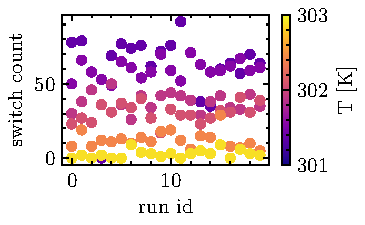
\includegraphics{bilder/plots/temp_comparison/switch_count_scatter.pdf}}
    \subcaptionbox{Mittel-, Extremwerte und Verteilung für jede Simulationstemperatur. Außerdem wurde der Wert auch aus der Kette an Simulationen berechnet (schwarze Punkte) \label{fig:temp-switch-count-violin}}{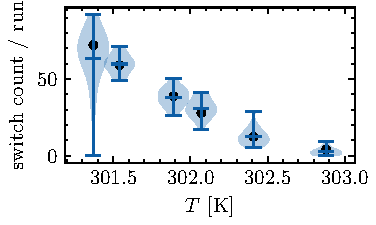
\includegraphics{bilder/plots/temp_comparison/switch_count_violin.pdf}}
    \caption{Temperaturabhängigkeit der Anzahl an Schaltvorgängen}\label{fig:temp-switch-count}
\end{figure}

\todo{Abb genauer Erklären und AUsreißerdatenpunkt diskutieren oder entfernen}

Die ansteigende Anzahl an Schaltvorgängen lässt sich auch in \cref{fig:temp-switch-count} gut erkennen. Außerdem sieht man in \cref{fig:temp-switch-count-scatter} einige Simulationsläufe, deren Werte aufgrund der Kurzen Simulationszeit (und daher teilweise das Telegrafenrauschen nicht immer korrekt extrahiert werden konnte) stark von den anderen abweichen.

Der aus der Kette berechnete Wert weicht auch jeweils nicht signifikant vom Mittelwert der aus den einzelnen Simulationen berechneten Werte ab.
Die kleinen Abweichungen lassen sich gut durch Probleme bei der Extraktion des Telegrafenrauschens bei einzenen Simulationsläufen (z.B. der 4. run bei \qnt{301}{\kelvin}) \todo{Satz beenden}


\begin{figure}[H]
    \centering
    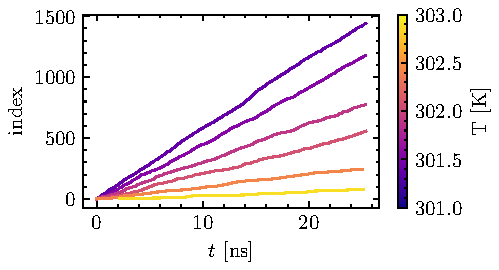
\includegraphics{bilder/plots/temp_comparison/switch_events.pdf}
    \caption{Zeitpunkt an dem ein Schaltvorgang stattfindet \todo{loglog achsen?}}\label{fig:switch-events}
\end{figure}

Die mittleren Aufenthaltszeiten (MDT) in den beiden Niveaus befinden sich in der gleichen Größenordnung, wie der Simulationszeitraum. Um auch bei weniger optimalen Daten, wie in \cref{fig:extraktion-tgr}, eine gute Extraktion des Telegrafenrauschens zu ermöglichen, wurden teilweise die Signale mehrerer Simulationsläufe hintereinander gehängt, um ein langes Signal zu erhalten.

Da aber nicht Zufälligerweise alle Simulationsläufe immer im gleichen Niveau starten und aufhören (so lange die Wahrscheinlichkeit für einen Zustand nicht deutlich höher ist), werden hierbei teilweise zusätzliche Schaltvorgänge hinzugefügt. 

Andere Möglichkeiten um die Rechenzeit zu verringern wären zum Beispiel eine eine größere Zeitschrittweite. Diese würde die Genauigkeit der Simulation verringern, sodass die Ergebnisse nicht mehr mit den experimentellen Daten vergleichbar wären. Bei einer Schrittweite von \qnt{100}{\femto\second} (wahrscheinlich aber schon früher) tritt das Telegrafenrauschen garnicht mehr auf und der Betrag der Magnetisierung ist deutlich größer.

\todo{ref anhang für verschiedene zeitschrittweiten}

\todo{andere Formulierung als lässt sich gut erkennen}
In \cref{fig:switch-events} lässt sich gut erkennen, dass die Schaltvorgänge gleichverteilt sind und Aufgrund der hohen Zahl an Schaltvorgängen, die zusätzlichen Schaltvorgänge durch die Verkettung nicht ins Gewicht fallen. \todo{satz in vorherigen Abschnitt eingliedern}


\begin{figure}[H]
    \centering
    \subcaptionbox{einzelner Datenpunkt für jede einzelne Simulation\label{fig:temp-up-percentage-scatter}}{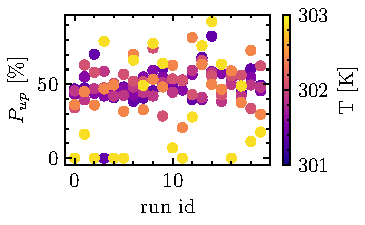
\includegraphics{bilder/plots/temp_comparison/up_percentage_scatter.pdf}}
    \subcaptionbox{Mittel-, Extremwerte und Verteilung für jede Simulationstemperatur. Außerdem wurde der Wert auch aus der Kette an Simulationen berechnet (schwarze Punkte)\label{fig:temp-up-percentage-violin}}{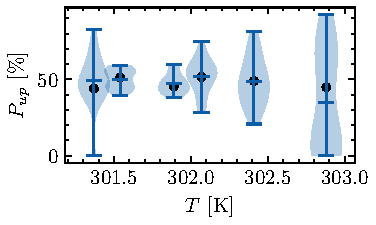
\includegraphics{bilder/plots/temp_comparison/up_percentage_violin.pdf}}
    \caption{Aufenthaltswahrscheinlichkeit im oberen Zustand}\label{fig:temp-up-percentage}
\end{figure}

Die Aufenthaltswahrscheinlichkeit für beide Zustände liegt in dem Temperaturbereich bei \qnt{50}{\percent}, aber für die Betrachtung der mittleren Aufenthaltszeit wird die Zahl der Simulationsläufe, in denen sich das System nur in einem Zustand befindet für höhere Temperaturen immer größer. Daher gibt es bei \qnt{303}{\kelvin} sehr viele Datenpunkte in \cref{fig:temp-up-percentage-scatter}, bei denen der aus einem Einzelnen Simulationslauf bereichnete Wert stark von \qnt{50}{\percent} abweicht.

\subsubsection{Spektrale Leistungsdichte und Autocovarianz}

\todo{Erklärrung, warum die Daten in der Zeitdomäne experimentell nicht messbar sind.}

\todo{wie misst man das experimentell überhaupt? (nur die Autocovarianz \(\gamma\) kann direkt bestimmt werden. darüber wird dann die Spektrale Leistungsdichte \(S\) berechnet)}

% Aufgrund der kurzen Zeitskalen (\unit{\femto\second})(\todo{und anderen Dingen?}) kann das magnetische Moment in c-Richtung Zeitlich aufgelöst so nicht beobachtet werden. Es ist aber möglich die Fouriertransformierte des Rauschsignals zu ermitteln und so das Phänomen zu charakterisieren. 

\begin{figure}[H]
    \centering
    \subcaptionbox{aus ursprünglichem Signal \label{fig:temp-spd-source}}{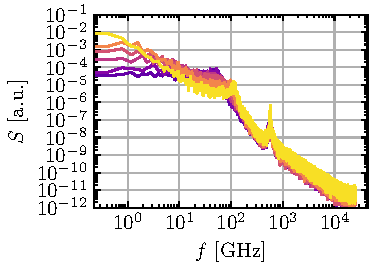
\includegraphics{bilder/plots/temp_comparison/spectral_power_density.pdf}}
    \subcaptionbox{aus bereinigtem Telegrafenrauschen \label{fig:temp-spd-clean}}{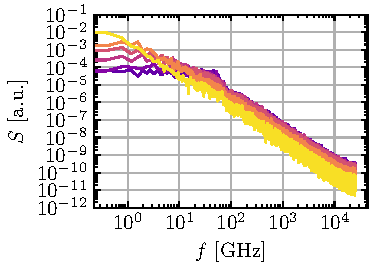
\includegraphics{bilder/plots/temp_comparison/spectral_power_density_cleaned.pdf}}
    \subcaptionbox{aus Differenz, bzw. statistischem Rauschen \label{fig:temp-spd-diff}}{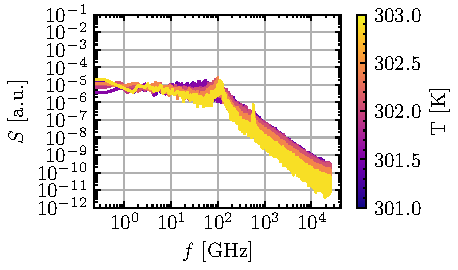
\includegraphics{bilder/plots/temp_comparison/spectral_power_density_diff.pdf}}
    \caption{Spektrale Leistungsdichten $S$ für verschiedene Temperaturen}\label{fig:temp-spd}
\end{figure}

Mit der Temperatuerhöhung verschiebt sich der  erste Eigenmode ( in \cref{fig:temp-spd-source}) nach rechts. 
Die Position des zweiten Eigenmode ändert sich nicht.


Die Spektrale Leistungsdichte des bereinigten Telegrafenrauschens (\cref{fig:temp-spd-clean}) ist bei höherer Temperatur im Niderfrequenten Bereich größer, aber fällt dann schneller ab.

Aus der Spektralen Leistungsdichte lässt sich die Autokorrelationsfunktion berechnen \cref*{eq:spd}.

\begin{figure}[H]
    \centering
    \subcaptionbox{aus ursprünglichem Signal\label{fig:temp-autocorr-source}}{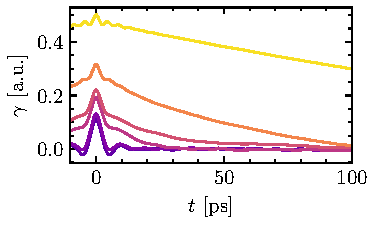
\includegraphics{bilder/plots/temp_comparison/autocorrelation.pdf}}
    \subcaptionbox{aus bereinigtem Telegrafenrauschen \label{fig:temp-autocorr-clean}}{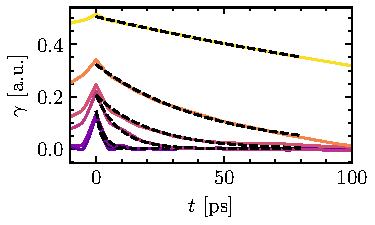
\includegraphics{bilder/plots/temp_comparison/autocorrelation_cleaned.pdf}}
    \subcaptionbox{aus Differenz, bzw. statistischem Rauschen \label{fig:temp-autocorr-diff}}{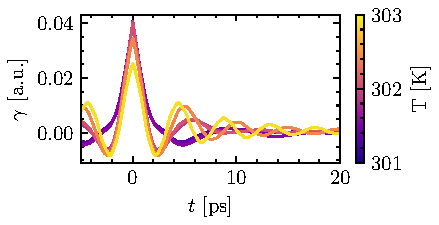
\includegraphics{bilder/plots/temp_comparison/autocorrelation_diff.pdf}}
    \caption{Autokorrelation $\gamma$ für verschiedene Temperaturen \todo{lieber fit bei source oder clean? besserer experimenteller vergleich vs. besseres Ergebnis. Die fits bei den unteren Temperaturen klappen bei beiden nicht.}}\label{fig:temp-autocorr}
\end{figure}

Da beide Zustände gleich wahrscheinlich sind konvergiert die Autokorrelationsfunktion für große Zeiten gegen 0 und ist daher identisch zur Autokovarianz. \todo{konvert das ganze bei hohen temperaturen wirklich gegen 0?}

\todo{charakteristische Abweichung von exponentiellem Abfall}

\begin{figure}[H]
    \centering
    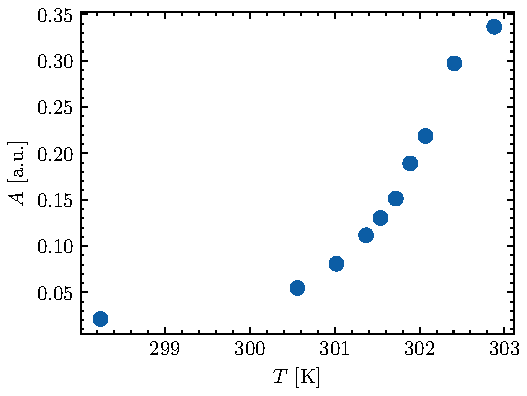
\includegraphics{bilder/plots/temp_comparison_long/rauschamplitude.pdf}
    \caption{Rauschamplitude $A$ für verschiedene Temperaturen $T$ \todo{Datenpunkte für T > 303K werden nicht berücksichtigt, weil autocov $\neq$ autocorr. die Rauschamplitude fällt aber ab}\todo{Exisiert eigentlich bereits in julius Masterarbeit. relevant für vergleich mit verhalten bei mit b-feld }}\label{fig:temp-autocorr-amplitude}
\end{figure}

Die Amplitude der Autokorrelationsfunktion steigt mit Erhöhung der Temperatur auch immer weiter an.

Aus Autokorrelationszeit lässt sich die mittlere Aufenthaltszeit für den symmetrischen DMP berechnen (\cref{eq:autokorr-sym-dmp}).


\todo{übergang Dominanz TGR}

\begin{figure}[H]
    \centering
    \subcaptionbox{Spektrale Leistungsdichten $S$ von ursprünglichem, bereinigtem Telegrafenrauschen und Differenz. Die Spektrale Leistungsdichte aus dem bereinigten Telegrafenrauschen wurde außerdem mit einem Lorentizan gefitted\label{fig:dominanz-spd}}{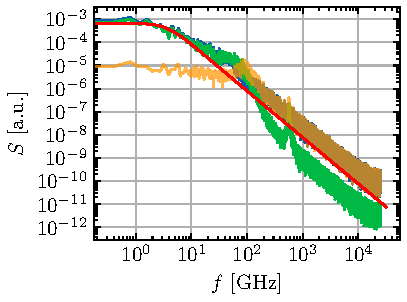
\includegraphics{bilder/plots/Bz_0mT/spectral_power_densities_26.03meV.pdf}}
    \subcaptionbox{Autokorrelation $\gamma$ von ursprünglichem, bereinigtem Telegrafenrauschen und Differenz. Die Autokorrelation aus dem bereinigten Telegrafenrauschen wurde außerdem mit einer exponentialfunktion gefitted \label{fig:dominanz-autocorr}}{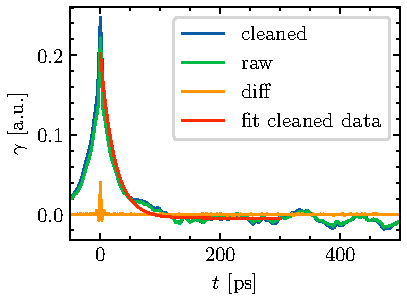
\includegraphics{bilder/plots/Bz_0mT/autocorr_26.03meV.pdf}}
    \caption{Dominanz des Telegrafenrauschen in der Frequenzdomäne. Simulation bei \qnt{26.03}{\milli\electronvolt} ohne externes Magnetfeld}\label{fig:dominanz-tgr}
\end{figure}

Beim direkten betrachten des Rauschsignals ist nicht klar erkennbar, ob das statistische oder das Telegrafenrauschen dominiert. Wenn man jedoch die Spektrale Leistungsdichte oder die Autokorrelation bzw. Autocovarianz betrachtet, ist deutlich erkennbar, dass das Telegrafenrauschen hier den größten Beitrag leistet.

\todo{Erklärung fits}

Aus dem in extrahiertem Telegrafenrauschen lassen sich die Aufenthaltszeiten im Zeitlichen Durchblick direkt herauslesen und mit den Berechneten Werten vergleichen. 

\begin{figure}[H]
    \centering
    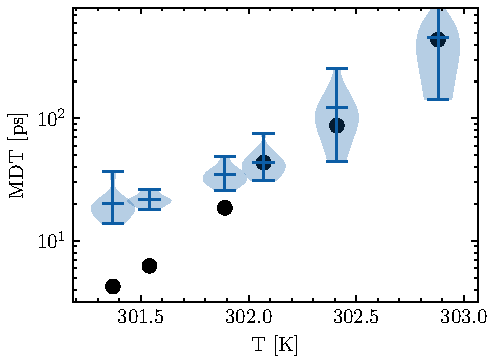
\includegraphics{bilder/plots/temp_comparison/mean_dwell_time_comparison.pdf}
    \caption{Mittlere Aufenthaltszeiten $MDT$ aus Zeitlicher Analyse (Violinenplot) und aus exponentiellem Fit der Autokorrelationsfunktion (schwarze Punkte) \todo{erwähnung, dass die Autokorrelationsfunktion aus den bereinigten Daten gefittet wurde}}\label{fig:temp-mdt-comp}
\end{figure}

Wie zu erwarten steigt die mittlere Aufenthaltszeit, bei einer höheren Temperatur an. Die auf die zwei verschiedenen Methoden berechneten Werte (und somit die bestimmte Anstiegsrate) weichen, bei niedrigeren Temperaturen, hier stark voneinander Ab. 
Wahrscheinlich liegt das an Problemen beim Fitten des exponentiellen Abfalls, Da für die niedrigen Temperaturen das charakteristische Verhalten\todo{was genau?} überwiegt.

\todo{Telegrafenrauschen nichtmehr dominant in Autokovarianz?}

Die Probleme beim Fitten des exponentiellen Abfalls sind in \cref{fig:temp-autocorr-fit} deutlich zu erkennen. Im Anfangsbereich ist die Fitfunktion bereits deutlich steiler, als die Autokorrelationsfunktion, um eine geringere Abweichung zu den späteren Datenpunkten zu haben (die selber nicht auf einem exponentiellen Verlauf liegen).

\todo{anderes fitintervall für niedrige temperaturen?}

\begin{figure}[H]
    \centering
    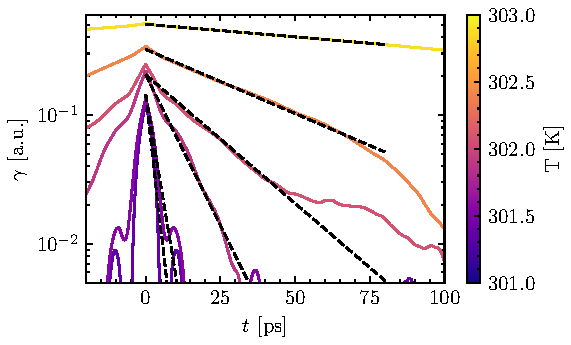
\includegraphics{bilder/plots/temp_comparison/autocorrelation_cleaned_log.pdf}
    \caption{Ausschnitt aus \cref{fig:bc-autocorr-clean}, in der versucht wird die Autokorrelation mit einer exponentialfunktion zu fitten. Hier aber in halblogarithmischer Darstellung}\label{fig:temp-autocorr-fit}
\end{figure}

\subsection{In externem Magnetfeld}

Das Verhalten des magnetischen Moments in c-Richtung kann nicht nur durch eine Veränderung der Temperatur beeinflusst werden, sondern auch durch ein extern angelegtes Magnetfeld.

\begin{figure}[H]
    \centering
    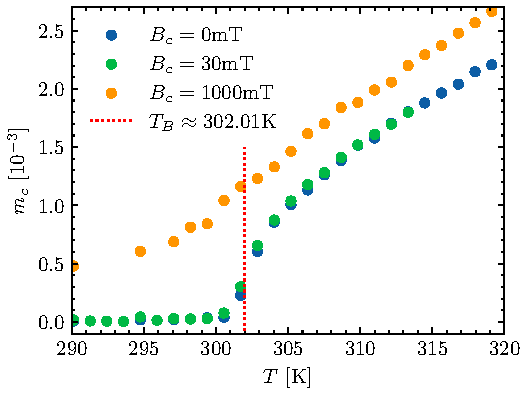
\includegraphics{bilder/plots/Bz_comparison/critical_temperature.pdf}
    \caption{Kritische Temperatur bei schwachem und starkem Magnetfeld in c-Richtung \todo{betrachtete Temperatur einzeichnen?}}\label{fig:bc-crit-temp}
\end{figure}

Bei einem starken Magnetfeld von \qnt{1}{\tesla} weicht der Reorientierungsübergang auf und es kommt kein Telegrafenrauschen, im Bereich von \num{300} bis \qnt{305}{\kelvin}, mehr zu Stande. Bei einem schwächeren Magnetfeld (um die \qnt{30}{\milli\tesla}) verändert sich die Position des Reorientierungsübergangs nicht signifikant. Daher wurden alle Simulationen mit angelegtem Magnetfeld bei der gleichen Temperatur durchgeführt.

% Das Magnetfeld wird in z-Richtung angelegt. Die c-Richtung im Kristall ist identisch zur z-Richtung im externen kartesischen Koordinatensystem.
% In den Simulationen wird auch immer nur ein konstantes Magnetfeld verwendet.
Als Temperatur wurde für jeden Simulationslauf \( \qnt{26.025}{\milli\electronvolt} \approx \qnt{302.01}{\kelvin}\) verwendet.
Der Simulationszeitraum beträgt für alle Simulationsläufe etwa \qnt{2.5}{\nano\s}

\begin{figure}[H]
    \centering
    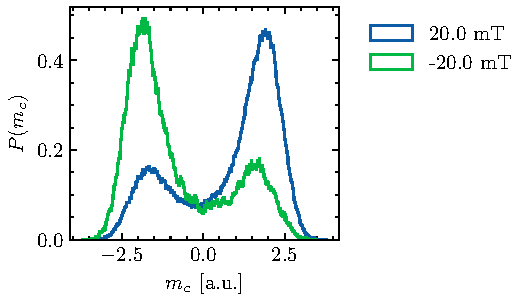
\includegraphics{bilder/plots/Bz_sign_comparison/20mT_hist_comp.pdf}
    \caption{Wahrscheinlichkeitsdichteverteilung von \(m_c\) bei einem externen Magnetfeld von \qnt{20}{\milli\tesla} mit entgegengesetzter Richtung}\label{fig:bc-sign-hist}
\end{figure}
\todo{Erleuterung/Epemplarische trajektorie (rauschen im Zeitlichen Verlauf)}

Das System scheint sich bei angelegtem B-Feld in entgegengesetzter Richtung Symmetrisch zu verhalten. Daher wurden die Simulationen nur mit positivem B-Feld durchgeführt.


\subsubsection{Betrachtung in der Zeitdomäne}

Auch hier lassen sich die Charakteristiken am schnellsten bei einer direkten statistischen Analyse des Signals erkennen.

\begin{figure}[H]
    \centering
    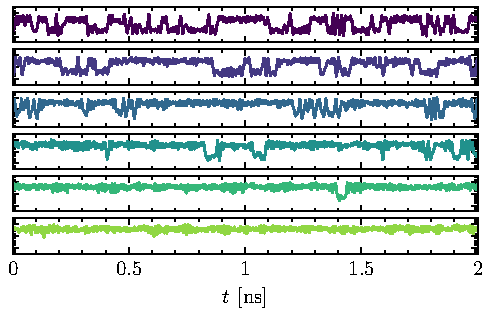
\includegraphics{bilder/plots/max_Bz/mc_time.pdf}
    \caption{Ausschnitt von \(m_c\) im Zeitlichen Verlauf bei verschieden starken externen Magnetfeldern . Die Colormap ist hier identisch zu der von \cref{fig:b-hist}. Die y-Achse reicht hier jeweils von \num{-1.5e-3} bis \num{+1.5e-3}}\label{fig:b-time}    
\end{figure}

\todo{Erläuterung}

\begin{figure}[H]
    \centering
    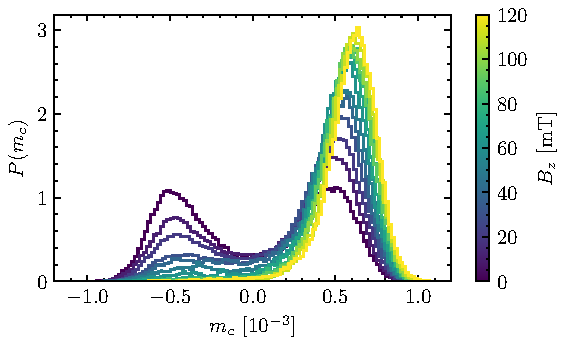
\includegraphics{bilder/plots/max_Bz/mc_hist.pdf}
    \caption{Wahrscheinlichkeitsdichteverteilung von \(m_c\) für eine Kombination von mehreren Simulationsläufen und bei verschieden starken externen Magnetfeldern}\label{fig:b-hist}    
\end{figure}

Anders als bei der Variation der Temperatur ohne externes Magnetfeld (\cref{fig:temp-hist}), sind die beiden Zustände nicht mehr Gleichverteilt. Wenn einer der beiden Peaks zu klein wird, kann der Algorithmus das Telegrafenrauschen nicht mehr extrahieren. 

Da das obere Niveau jetzt aber eine deutlich höhere Aufenthaltswahrscheinlichkeit hat, kommt es auch (je nach stärke des B-Feldes) zu deutlich weniger zusätzlichen Schaltvorgängen bei der Verkettung mehrerer Simulationsläufe.

\todo{erklärung verschiebung der Niveau peaks}

\begin{figure}[H]
    \centering
    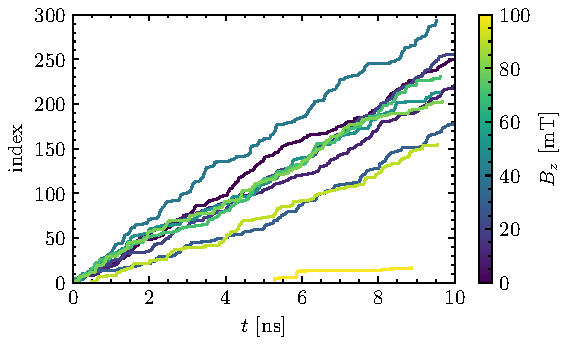
\includegraphics{bilder/plots/max_Bz/switch_events.pdf}
    \caption{Zeitpunkt an dem ein Schaltvorgang stattfindet}\label{fig:bc-switch-events}   
\end{figure}

\todo{hier bei 100mT garantiert kein problem aufgrund der Verkettung, da sich das system quasi durchgängig im oberen Niveau befindet}

In Manchen Simulationsläufen bei \qnt{100}{\milli\tesla} findet gar kein Schaltvorgang statt. \todo{mehr roten Faden}

\todo{vergleich mit \cref{fig:switch-events} }

Ähnlich wie in \cref{fig:switch-events} sind die Zustandswechsel recht gleichverteilt. Bei einer höheren Temperatur sind deutlichere Stufen erkennbar, da häufiger auf einen Schaltvorgang direkt ein zweiter (zurück in den energetisch begünstigten Zustand) stattfindet. Die Rate an Zustandswechseln bleibt jedoch im Rahmen der Unsichheiten konstant. Erst wenn quasi keine Zustandswechsel mehr stattfinden, weicht dieser Wert signifikant von denen bei niedrigeren Feldstärken ab. 

\begin{figure}[H]
    \centering
    \subcaptionbox{Aufenthaltszeit im oberen Zustand. Bestimmt über einzelne Simulationsläufe (Violinplot) und über Kette mehrerer Simulationen (schwarze Punkte) \label{fig:bc-up-percentage-violin}}{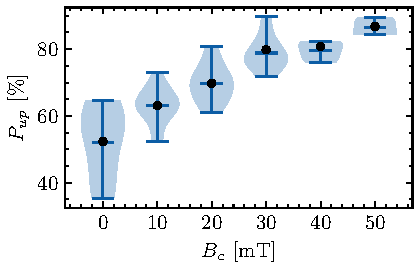
\includegraphics{bilder/plots/max_Bz/up_percentage_violin.pdf}}
    \subcaptionbox{Mittlere Aufenthaltszeit in oberem (blau) und unterem (grün) Zustand in Prozent. Die wagrechte Linie kennzeichnet hierbei den Mittelwert und der Violinplot die Verteilung der verschiedenen Aufenthaltszeiten auf dem jeweiligen Niveau  \todo{Abweichung up 40mT erklären/beheben?}\label{fig:bc-state-times-comp}}{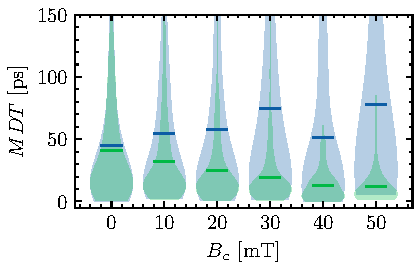
\includegraphics{bilder/plots/max_Bz/state_times_comp.pdf}}
    \caption{Abhängigkeit der Aufenthaltszeit von der Magnetfeldstärke}\label{fig:bc-state-times}
\end{figure}

Was sich allerdings stark ändert ist die Aufenthaltswahrscheinlichkeit und mittleren Aufenthaltszeiten für die beiden Niveaus.

\todo{Diskussion Aufenthaltswahrscheinlichkeit}

\todo{diskussion mittlere Aufenthaltszeiten}

\begin{figure}[H]
    \centering
    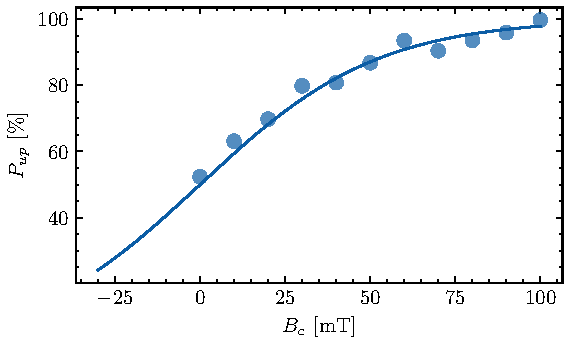
\includegraphics{bilder/plots/max_Bz/up_percentage_fit.pdf}
    \caption{Die Aufenthaltszeit im oberen Zustand mit einer Sigmoid-Funktion gefittet. Die Datenpunkte wurden dabei mittels des Algorithmus aus mehreren verketteten Simulationsläufen extrahiert}\label{fig:bc-up-percentage}
\end{figure}

Aus mehreren verketteten Simulationsläufen ist es möglich auch für höhere Feldstärken als in \cref{fig:bc-up-percentage-violin} die Aufenthaltswahrscheinlichkeit zu bestimmen. Diese folgt einer Sigmoid-Kurve.\todo{muss erklärt werden?} Oberhalb von \qnt{100}{\milli\tesla} findet in den Simulationen kein Telegrafenrauschen mehr statt.

\todo{worin ist das sonst erkennbar, dass kein Schaltvorgang mehr stattfindet?}

\subsubsection{Spektrale Leistungsdichte und Autokovarianz}

\todo{Hinsichtlich des Experiments sind  ... besonders interessant}
% Da die Analyse im zeitlichen Durchblick hier experimentell leider nicht möglich ist, müssen Anhaltspunkte im Frequenzdurchblick gefunden werden um u.a. festzustellen, wann kein Telegraphenrauschen mehr stattfindet.

\begin{figure}[H]
    \centering
    \subcaptionbox{aus ursprünglichem Signal\label{fig:bc-spd-source}}{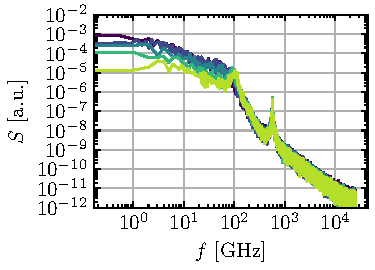
\includegraphics{bilder/plots/max_Bz/spectral_power_density.pdf}}
    \subcaptionbox{aus bereinigtem Telegrafenrauschen\label{fig:bc-spd-clean}}{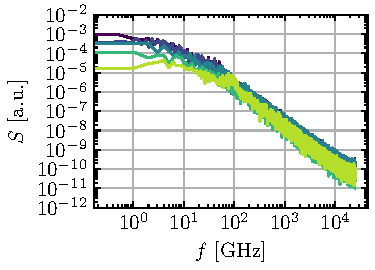
\includegraphics{bilder/plots/max_Bz/spectral_power_density_cleaned.pdf}}
    \subcaptionbox{aus Differenz, bzw. statistischem Rauschen \label{fig:bc-spd-diff}}{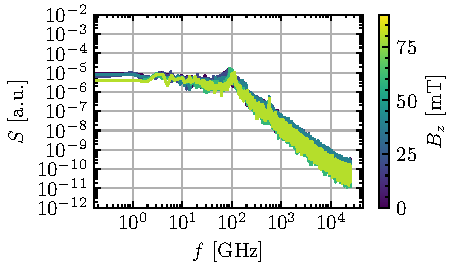
\includegraphics{bilder/plots/max_Bz/spectral_power_density_diff.pdf}}
    \caption{Spektrale Leistungsdichten $S$ bei verschiedenen Magnetfeldstärken}\label{fig:bc-spd}
\end{figure}

So wie bei der Erhöhung der der Temperatur in \cref{fig:temp-spd-source} zu einer Verschiebung des ersten Peaks geführt hat, führt in  \cref{fig:bc-spd-source} eine erhöhung der Feldstärke auch zu einer verschiebung des Peaks nach rechts. Der zweite Peak bleibt auch unverändert.\todo{die Peaks heißen Eigenmoden}

Die spektrale Leistungsdichte ist allerdings im niederfrequenten Bereich in \cref{fig:bc-spd-source,fig:bc-spd-clean} bei größerer Feldstärke deutlich geringer und bleibt in \cref{fig:bc-spd-clean} auch kleiner im Vergleich zu den anderen Kurven.

\todo{Aber TGR Dominiert für niedrige Frequenzen}

\begin{figure}[H]
    \centering
    \subcaptionbox{aus ursprünglichem Signal \label{fig:bc-autocorr-source}}{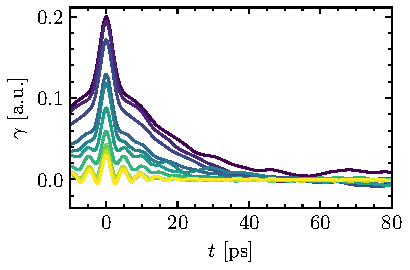
\includegraphics{bilder/plots/max_Bz/autocov.pdf}}
    \subcaptionbox{aus bereinigtem Telegrafenrauschen\label{fig:bc-autocorr-clean}}{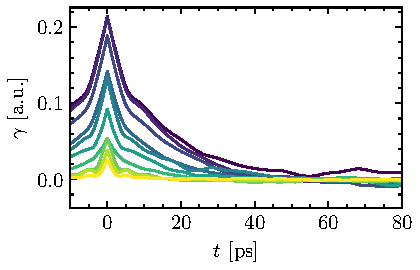
\includegraphics{bilder/plots/max_Bz/autocov_cleaned.pdf}}
    \subcaptionbox{aus Differenz, bzw. statistischem Rauschen\label{fig:bc-autocorr-diff}}{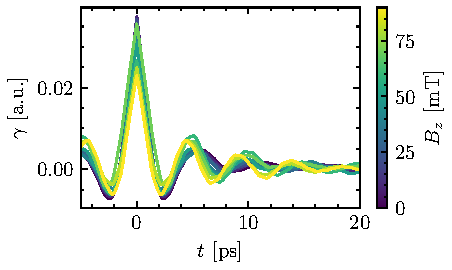
\includegraphics{bilder/plots/max_Bz/autocorrelation_diff.pdf}}
    \caption{Autokovarianz $\gamma$ für verschiedene Magnetfeldstärken }\label{fig:bc-autocov}
\end{figure}

\todo{Autokorrelation vs Autokovarianz}

Die Autokorrelationsfunktionen konvergieren bei externem Magnetfeld nichtmehr gegen \num{0} (da die beiden Zustände eine unterschiedliche Aufenthaltswahrscheinlichkeit haben). Daher musste, um die Autokovarianzkurven in \cref{fig:bc-autocov} zu erhalten, der Grenzwert von der Autokorrelationsfunktion abgezogen werden.

Die mittlere Aufenthaltszeit ist aus dem gleichen Grund auch nichtmehr aus der Autokovarianz bestimmbar. 

% Wann der exponentielle Abfall (Abbild \todo{wie lautet korrekter Fachbegriff?} des Telegrafenrauschen in der Autokorrelation) nichtmehr mit den anderen Charakteristika \todo{haben die einen Namen?} überlagert ist lässt sich auch direkt aus der Autokorrelation des rohen Signals erkennen:

% \begin{figure}[H]
%     \centering
%     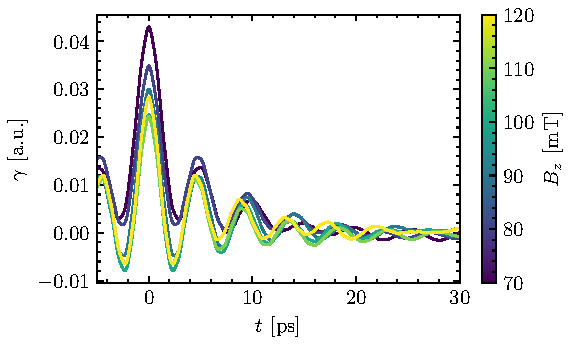
\includegraphics{bilder/plots/max_Bz/autocov_high.pdf}
%     \caption{Autokovarianz $\gamma$ für hohe Magnetfeldstärken (dem entsprechend ändert sich auch wieder die Skala der colormap)}\label{fig:bc-autocov-high}
% \end{figure}

% Die Autokovarianzkurven für die Feldstärken \qnt{\geq 90}{\milli\tesla} (bei denen quasi kein telegrafenrauschen mehr stattfindet) liegen fast 
% perfekt übereinander. 

% Um dieses Verhalten zu parametrisieren reicht es aus die Rauschamplitude \(\gamma(0)\) zu betrachten:

\begin{figure}[H]
    \centering
    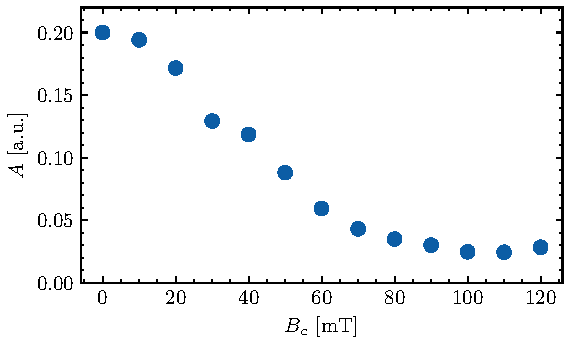
\includegraphics{bilder/plots/max_Bz/rauschamplitude.pdf}
    \caption{Amplitude der Autokovarianz abhängig von \(B_z\)}\label{fig:bc-rauschampl}
\end{figure}

Die Amplitude der Autokovarianz wird bei Erhöhung der Temperatur immer kleiner und oberhalb von \qnt{100}{\milli\tesla} minimal.
% Sie scheint danach wieder anzusteigen, Die Abweichung des Datenpunktes bei \qnt{120}{\milli\tesla} ist aber alleine nicht aussagekräftig. 

\todo{warum fällt die Rauschamplitude ab?}

% bibliography (temporary)
% \bibliography{literatur} \todo{comment out before compiling main.tex}

\end{document}